
%(BEGIN_QUESTION)
% Copyright 2011, Tony R. Kuphaldt, released under the Creative Commons Attribution License (v 1.0)
% This means you may do almost anything with this work of mine, so long as you give me proper credit

This Allen-Bradley SLC 500 PLC program writes data to a variable-frequency drive using Modbus protocol.  The PLC receives data from an HMI panel in the form of an integer value and a momentary ``ENTER pushbutton'' bit signal (writing to bit {\tt B3:0/5} in the PLC).  It is important to note that MicroLogix programs such as this one require a ``one-shot'' to drive any communication instructions such as {\tt MSG}.  If a {\tt MSG} instruction is continually activated in a ladder-logic program it experiences trouble completing its task, as though each fresh scan of the program interrupts the instruction's action begun on the previous scan:


$$\includegraphics[width=15.5cm]{i04531x01.eps}$$

Explain how this program functions, especially how the ``one-shot'' ({\tt ONS}) instruction prevents the {\tt MSG} instruction from ``talking over itself''.  How many integer registers are used in the SLC 500 PLC's memory for storing data relevant to the MSG instruction?  What type(s) of data are being written to the VFD?

\vskip 10pt

Presently this program sends a Modbus message to another device once for every positive transition of the {\tt B3:0/5} bit.  Suppose you wished to alter this program so that it transmits a Modbus message regularly every half-second or so.  How could you edit the program to do this?

\vskip 10pt

A lot of details seem to be missing from this instruction as it appears in the RSLogix 500 software display.  Identify some of the pertinent parameters we do {\it not} see in this MSG instruction, and where the human programmer could navigate to in the RSLogix software to view them.

\underbar{file i04531}
%(END_QUESTION)





%(BEGIN_ANSWER)

\noindent
{\bf Partial answer:}

\vskip 10pt

In order to alter the program for regular Modbus message transmissions, you can replace the {\tt B3:0/5} contact instruction with a contact instruction linked to one of the {\tt S:4} status bits (a continually counting binary number in the Allen-Bradley PLC's free-running clock).  Choose whichever status bit toggles at a frequency closest to 2 Hz (once every half-second).

%(END_ANSWER)





%(BEGIN_NOTES)

When bit {\tt B3:0/5} transitions from low to high (0 to 1), the MSG instruction is activated.  According to the Allen-Bradley SLC 500 instruction set manual, you must trigger the MSG instruction {\it once} per use.

\vskip 10pt

In order to alter the program for regular Modbus message transmissions, you can replace the {\tt B3:0/5} contact instruction with a contact instruction linked to one of the {\tt S:4} status bits (a continually counting binary number in the Allen-Bradley PLC's free-running clock).  Choose whichever status bit toggles at a frequency closest to 2 Hz (once every half-second).

\vskip 10pt

The Setup Screen for the MSG instruction prompts entry of the following parameters (all necessary for operation):

\begin{itemize}
\item{} {\bf Parameters for PLC:}
\item{} Data table address (memory location in PLC for communicated data)
\item{} Size in Elements (how many words of data will be communicated)
\item{} Channel (serial, Ethernet, etc.)
\vskip 10pt
\item{} {\bf Parameters for Target Device:}
\item{} Message timeout
\item{} Data table address (memory location in target device for communicated data)
\item{} Data table offset
\item{} Local Node Address (serial network address of the target device)
\item{} Ethernet (IP) Address (Ethernet network address of the target device)
\item{} MultiHop (whether or not communication happens directly between two devices)
\item{} {\it various network ``Bridge'' parameters}
\end{itemize}

%INDEX% PLC, ladder logic program analysis and explanation (Allen-Bradley SLC 500)

%(END_NOTES)


